 \begin{figure}[h!]
    \centering
    \begin{subfigure}[b]{0.23\textwidth}
        \centering
        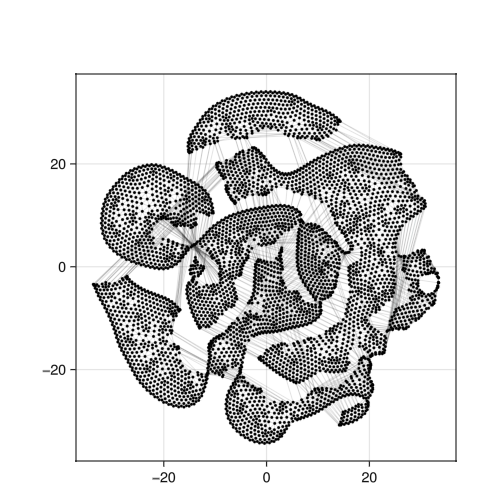
\includegraphics[trim={0 0 0 2.5cm}, clip, width=1.1\textwidth]{images/plot_ex_1.png}
        % \caption{}
        \label{fig:visu_simple}
    \end{subfigure}
    \hfill
    \begin{subfigure}[b]{0.23\textwidth}
        \centering
        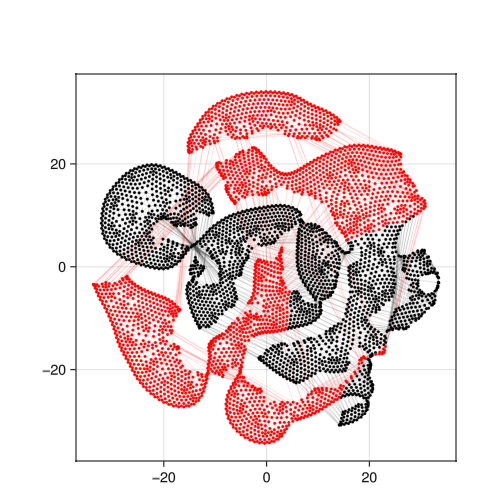
\includegraphics[trim={0 0 0 2.5cm}, clip, width=1.1\textwidth]{images/plot_ex_2.png}
        % \caption{}
        \label{fig:visu_2part}
    \end{subfigure}
    \caption{Graph visualization example and the corresponding result after applying
    a bisection. The original graph structure is shown on the left, while the right 
    visualization highlights the two obtained partitions.}
    \label{fig:visu}
\end{figure}